\documentclass{article}
\usepackage[utf8]{inputenc}
\usepackage[russian]{babel}
\usepackage{graphicx}
\usepackage{amsmath}
\usepackage{breqn}
\usepackage{wrapfig}
\usepackage{float}
\usepackage{multirow}
\usepackage{caption}
\usepackage{subcaption}

\graphicspath{ {./data/images} }
\author{Александр Романов Б01-107}
\date{}
\title{3.5.1 Изучение плазмы газового разрда в неоне}

\begin{document}
\maketitle
\section{Введение}
\subsection{Цель работы}
Изучение вольт-амперной характеристики тлеющего разряда; Изучение свойств плазмыметодом зондовых
характеристик.
\subsection{В работе используются} 
Стеклянная газоразрядная трубка, наполненная неоном; Высоковольтный источник питания; Источник
питания постоянного тока; Делитель напряжения; Потенциометр; Амперметры; Вольметры; переключатели.
\begin{figure}[H]
    \centering
    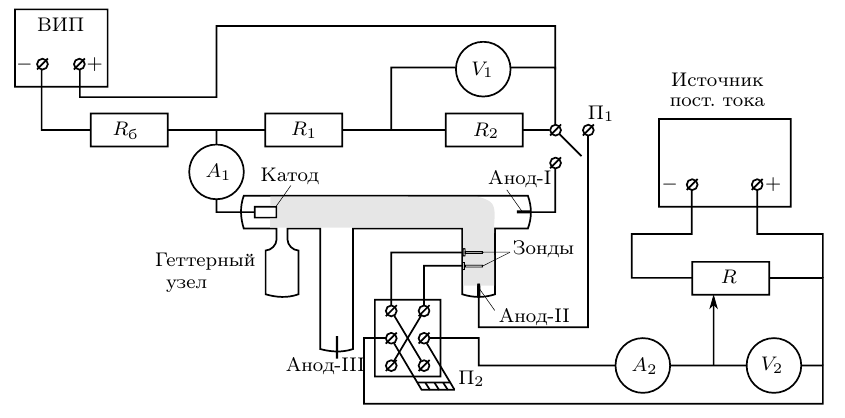
\includegraphics[width=0.8\textwidth]{sheme.png}
    \caption{Схема установки для исследования газового разряда}
\end{figure}

\section{Работа}
\subsection{Вольт-амперная характеристика разряда}
Установим переключатель \(\text{П}_1\) в положение "Анод-I". Установим напряжение, подаваемое с ВИП в 0.
Плавно увеличивая выходное напряжение ВИП, определим напряжение зажигания разряда \(V_{d}\) (По
показания вольиетра \(V_1\) непосредственно перед зажиганием). Получим: \(V_{d} = 230\; V\)

Снимем с помощью вольтметра \(V_1\) и амперметра \(A_1\) ВАХ разряда \(I_{d}\left(V_{d}\right)\). 
Изменять ток разряда \(I_{dsch}\) будем в диапазоне \(\left(0.5\; mA - 5\; mA\right)\). 

\begin{table}[H]
    \centering
    \begin{tabular}{|c|c|}
    \hline
    U, V  & I, mA \\\hline
    32    & 1.4   \\\hline
    31.9  & 1.8   \\\hline
    28.7  & 2.28  \\\hline
    27.8  & 2.8   \\\hline
    26.9  & 3.28  \\\hline
    25.7  & 3.8   \\\hline
    24.9  & 4.28  \\\hline
    24.4  & 4.8   \\\hline
    25    & 4.28  \\\hline
    25.6  & 3.8   \\\hline
    26.9  & 3.32  \\\hline
    27.6  & 2.8   \\\hline
    28.3  & 2.32  \\\hline
    31.96 & 1.8   \\\hline
    33.2  & 1.28  \\\hline
    34.3  & 0.8   \\\hline
    35    & 0.46  \\\hline
    \end{tabular}
\end{table}

\begin{figure}[H]
    \centering
    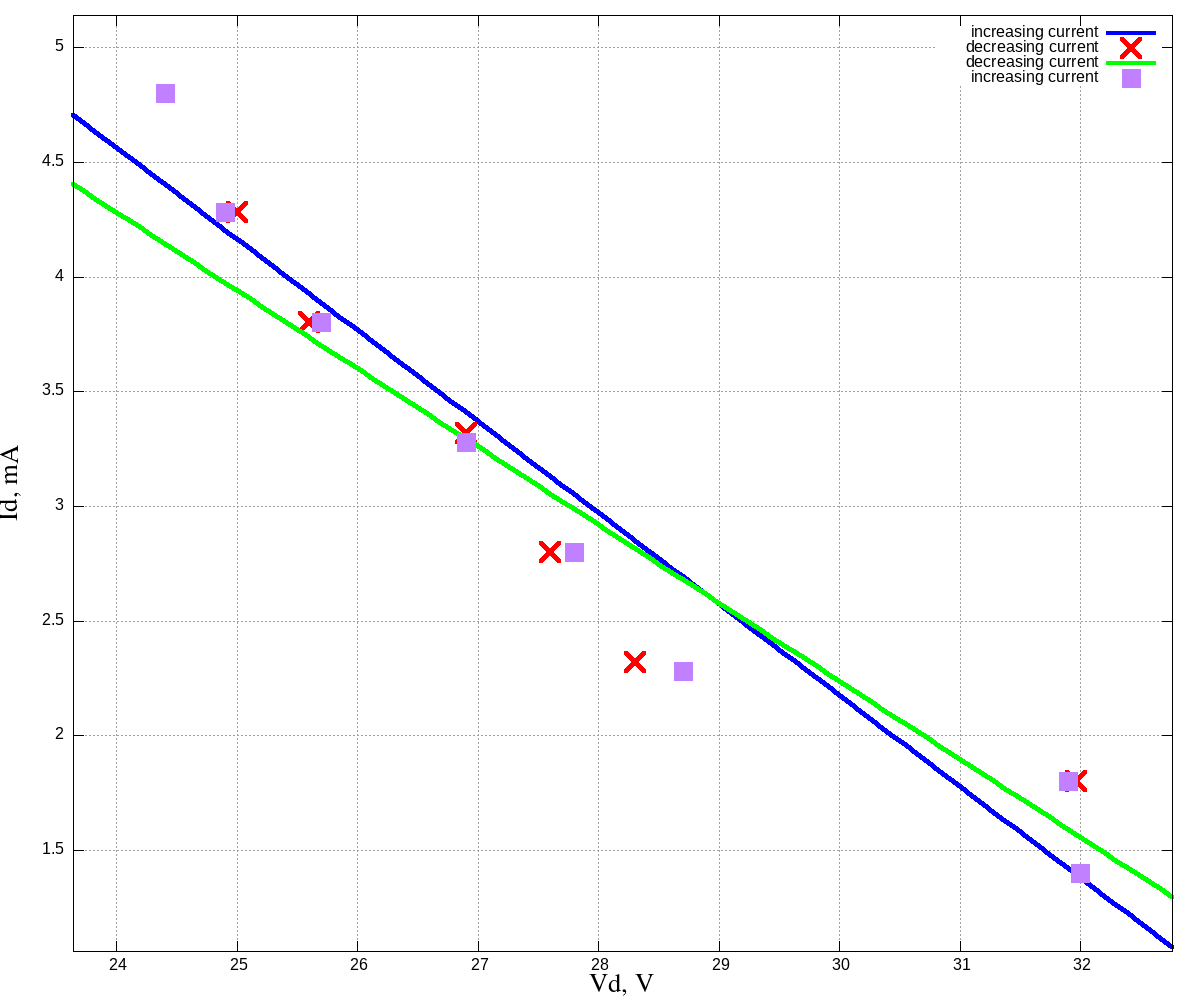
\includegraphics[width=\textwidth]{V-A-1.png}
\end{figure}

Опроксимировав уравнением (\(y = kx + b\)) получим уравнения для уменьшения тока:
\[ k = (-0.34 \pm 0.02)\; mA/V \]
\[ b = (12.5 \pm 0.08)\; mA \]

И для повышения тока:
\[ k = (-0.40 \pm 0.03)\; mA/V \]
\[ b = (14.1 \pm 0.09)\; mA \]

Как видно из графиков, прямые очень похожи. По их наклону определим дифференциальное сопротивление разряда:
\[ R_{diff} = \frac{dV}{dI} = (-2.5 \pm 0.18)\cdot 10^{3}\: \Omega \]

\subsection{Зондовые характеристики}
Уменьшим напряжение ВИП до 0. Переведём переключатель \(\text{П}_1\) в положение "Анод-II",
переключатель \(\text{П}_2\) в положение "+".
Плавно увеличим напряжение ВИП и установим разрядный ток \(I_d = 5\:mA\). Включим в сеть источник
питания постоянного тока и установим на нем выходное напряжение \(V_2 = 25\:V\). При помощи
потенциометра \(R\) установим на зонде максимальное напряжение \(V_@ = 25\:V\).
С помощью амперметра \(A_2\) и вольметра \(V_2\) снимем ВАХ двойного зонда \(I_3\left(V_3\right)\).
Измерим ВАХ также при \(I_d = 3\: mA\) и \(I_d = 1.5\: mA\)

\begin{table}[H]
    \centering
    \begin{tabular}{|c|c|c|c|c|c|}
    \hline
    \multicolumn{2}{|c|}{\(I_d = 5\: mA\)}& \multicolumn{2}{|c|}{\(I_d = 3\: mA\)} & \multicolumn{2}{|c|}{\(I_d = 1.5\: mA\)} \\\hline
    \(V_3,\; V\) & \(I_3,\: mA\) & \(V_3,\; V\) & \(I_3,\: mA\) & \(V_3,\; V\) & \(I_3,\: mA\)\\\hline
    25 & 103  & 25          & 55& 25           & 27 \\\hline
    22 & 100  & 22          & 54& 22           & 26 \\\hline
    19 & 98   & 19          & 52& 19           & 25 \\\hline
    16 & 95   & 16          & 50& 16           & 24 \\\hline
    13 & 91   & 13          & 48& 13           & 23 \\\hline
    10 & 82   & 10          & 45& 10           & 21 \\\hline
    8  & 74   & 8           & 40& 8            & 19 \\\hline
    6  & 62   & 6           & 34& 6            & 16 \\\hline
    4  & 49   & 4           & 26& 4            & 12 \\\hline
    2  & 31   & 2           & 14& 2            & 6.5\\\hline
    0.6& 18   & 0.6         & 6 & 0.6          & 2  \\\hline
    -0.6 &17  & -0.6        & 4 & -0.6         & 2  \\\hline
    -2 & 29   & -2          & 13& -2           & 6  \\\hline
    -4 & 49   & -4          & 24& -4           & 12 \\\hline
    -6 & 63   & -6          & 34& -6           & 16 \\\hline
    -8 & 75   & -8          & 41& -8           & 19 \\\hline
    -10& 85   & -10         & 47& -10          & 22 \\\hline
    -13& 94   & -13         & 50& -13          & 24 \\\hline
    -16& 100  & -16         & 53& -16          & 25 \\\hline
    -19& 103  & -19         & 55& -19          & 26 \\\hline
    -22& 106  & -22         & 56& -22          & 27 \\\hline
    -25& 109  & -25         & 58& -25          & 28 \\\hline
    \end{tabular}
\end{table}

\subsubsection*{\(I_d = 5\: mA\):}
\begin{figure}[H]
    \centering
    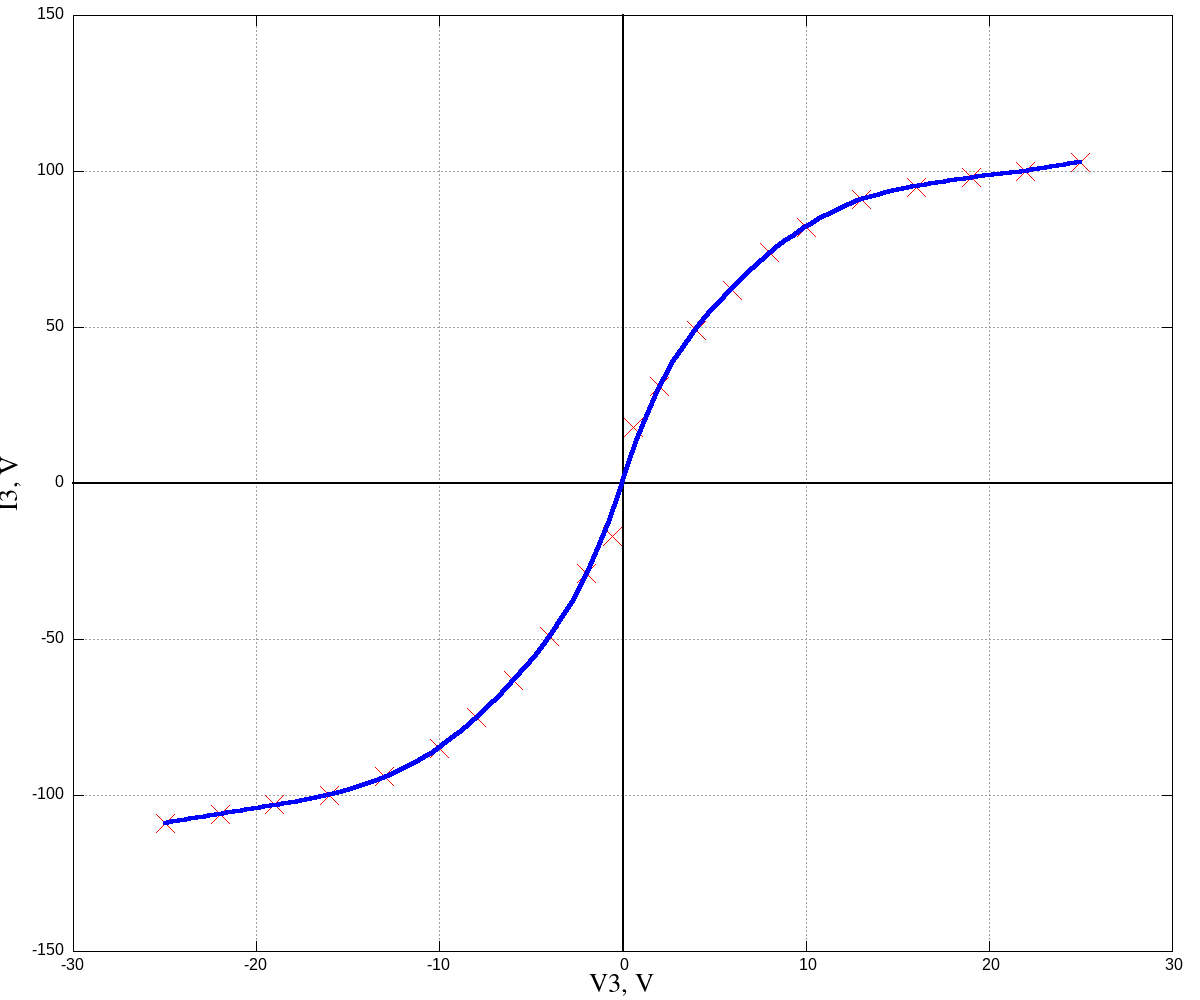
\includegraphics[width=0.8\textwidth]{V-A-5.png}
\end{figure}

\subsubsection*{\(I_d = 3\: mA\):}
\begin{figure}[H]
    \centering
    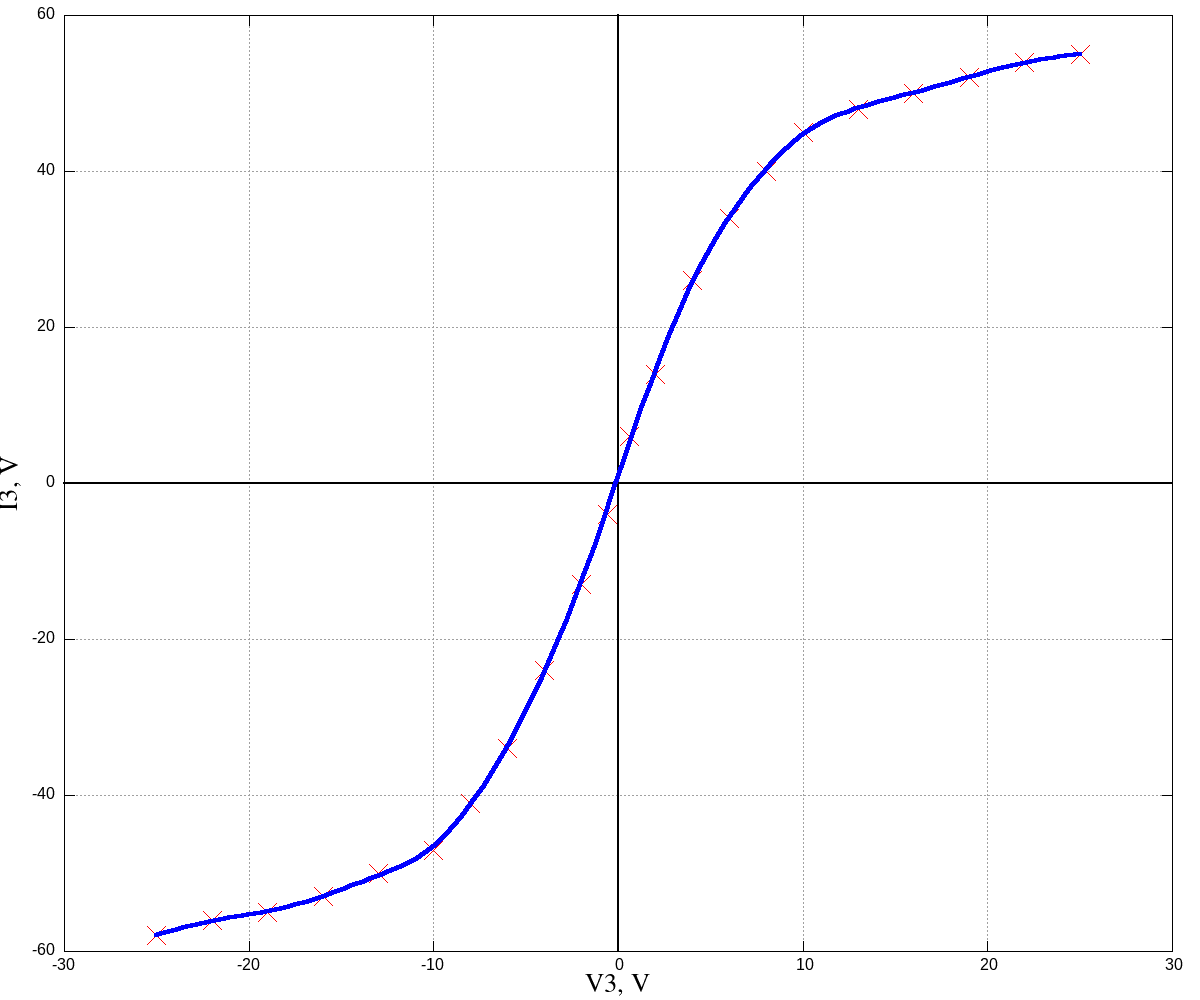
\includegraphics[width=0.8\textwidth]{V-A-3.png}
\end{figure}

\subsubsection*{\(I_d = 1.5\: mA\):}
\begin{figure}[H]
    \centering
    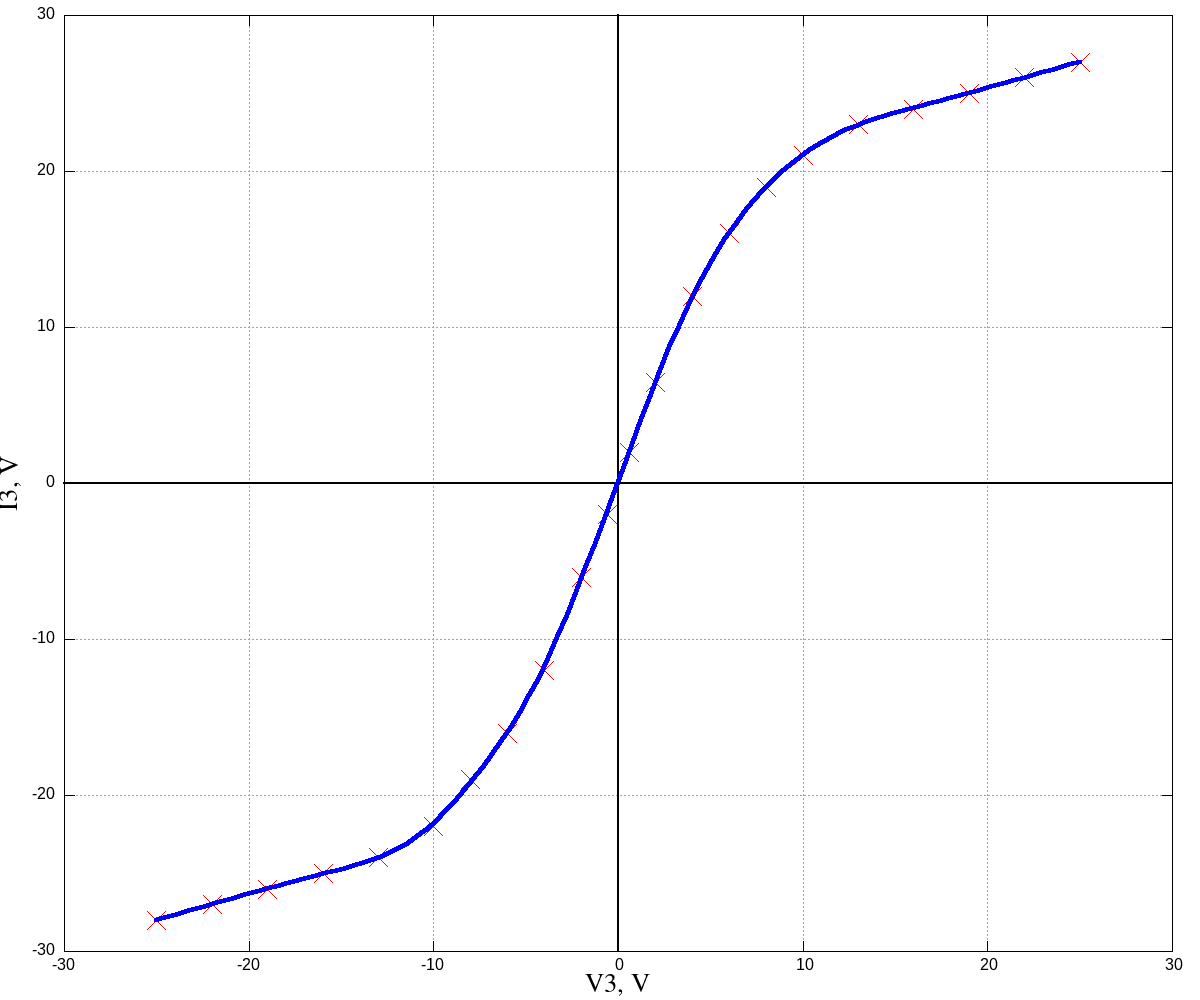
\includegraphics[width=0.8\textwidth]{V-A-1.5.png}
\end{figure}

По ВАХ для всех трёх значений \(I_d\) легко убедиться что участки кривой при больших напряжениях
выходят на асимптоты.



\section{Выводы}


\end{document}